\documentclass{pdfmx4020}
%\documentclass{mx4020}
\usepackage{hyperref}

\Title{your title}
\Author{your name}
\Year{2013--2014}
\Supervisor{your supervisor}

\begin{document}

\mxfrontpage

\begin{Summary}
Enter your summary here ...
\end{Summary}

\StartThesis

\chapter{chapter title}
Some content ...

\begin{lemma}  
Here is a lemma
\end{lemma}

\begin{definition}  
Here is a definition\cite{c1}
\end{definition}

\begin{theorem}  
Here is a theorem
\end{theorem}

\begin{corollary}  
Here is a corollary
\end{corollary}

\begin{example}  
Here is a example
\end{example}

\begin{remark}  
Here is a remark
\end{remark}

Here is an example of an equation.
\begin{equation*}  
y = x^2
\end{equation*}

Here is an example figure.
\begin{figure}[htbp]
	\centering
		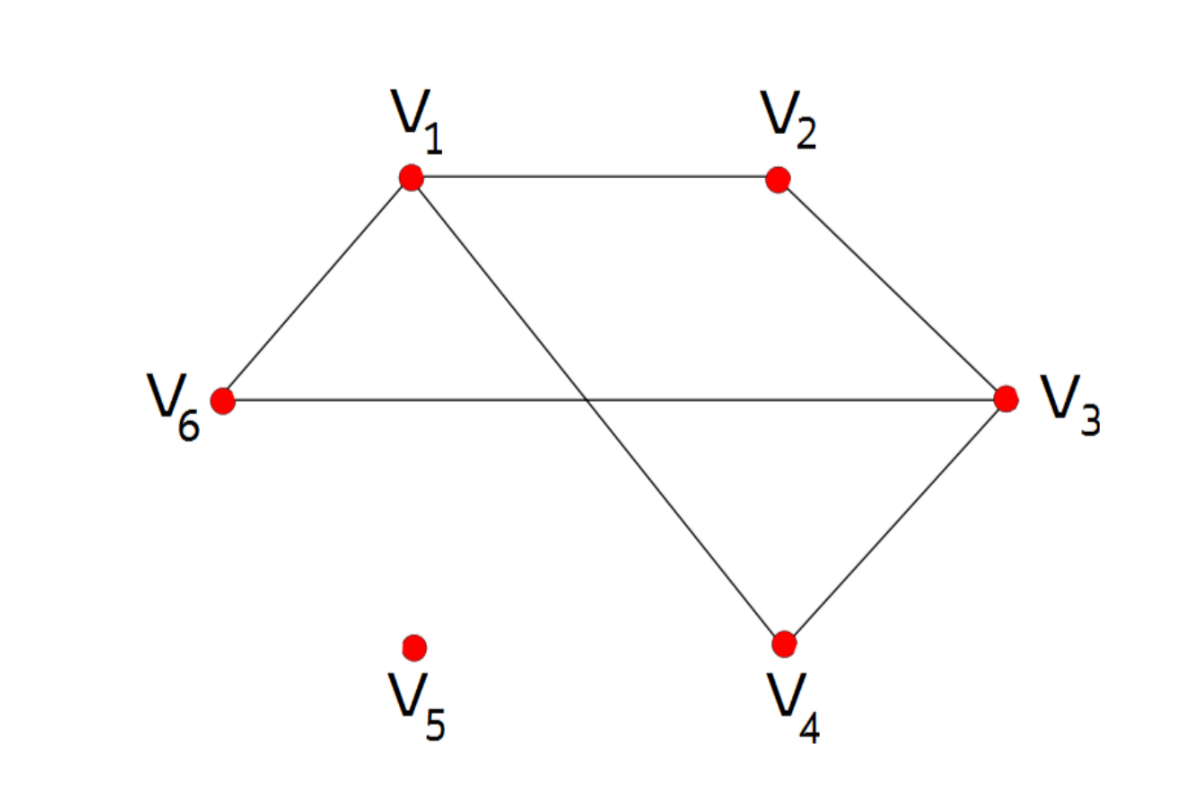
\includegraphics[width=0.50\textwidth]{graph.png}
	\caption{Some caption text}
	\label{fig:graph}
\end{figure}

%this is a table
\begin{tabular}{|r|l|}
  \hline
  7C0 & hexadecimal \\
  3700 & octal \\ \cline{2-2}
  11111000000 & binary \\
  \hline \hline
  1984 & decimal \\
  \hline
\end{tabular}

\section{section title}
Some more content ...

\subsection{subsection title}
Some more content ...

\chapter{the next chapter}
Some more content ...

\begin{thebibliography}{999}

\bibitem{c1} Jones, A., Smith, B. 2004.\emph{book/article title}. other publication details

\end{thebibliography}

\end{document}
